\documentclass[12pt]{article}

% report, book

%  Русский язык

\usepackage[T2A]{fontenc}
\usepackage[utf8]{inputenc}
\usepackage[english,russian]{babel}

\usepackage{amsmath,amsfonts,amssymb,amsthm,mathtools} 

\usepackage{graphicx}
\usepackage{listings}
\usepackage{hyperref}
\usepackage[table,xcdraw]{xcolor}

\usepackage{wasysym}

\usepackage{geometry} 
\geometry{a4paper,top=2cm,bottom=3cm,left=2cm}

\begin{document}

\begin{titlepage}
   \begin{center}
       \vspace*{1cm}

       \textbf{Лабораторная работа №1}

       \vspace{0.5cm}
        Алгоритмы одномерной минимизации функции
            
       \vspace{1.5cm}

       \textbf{Сысоев Александр, Зырянова Мария}
       
       \textbf{Верблюжий случай}

       \vfill
            
   \end{center}
\end{titlepage}

\section{Постановка задания}

Необходимо реализовать алгоритмы одномерной минимизации функции:

\begin{itemize}
\item метод дихотомии
\item метод золотого сечения
\item метод Фиббоначи
\item метод парабол
\item комбинированный метод Брента
\end{itemize}

\section{Исследуемая функция}

Необходимо на интервале $[0.1; 2.5]$ найти минимум функции 

\begin{equation*}
f(x)=10xln(x)-\frac{x^2}{2}
\end{equation*}

$x_0$ -- точка локального экстремума $f(x)$, если $f'(x_0) = 0$:

\begin{equation*}
f'(x)=10+10ln(x)-x=0
\end{equation*}

\begin{figure}[h]
\centering
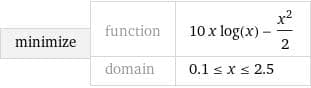
\includegraphics[width=0.5\textwidth]{images/problem.jpg}
\caption{Нахождение локального минимума при помощи WolframAlpha}
\end{figure}

\begin{figure}[h]
\centering
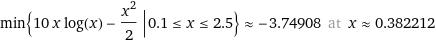
\includegraphics[width=0.5\textwidth]{images/solution.jpeg}
\caption{Найденное решение}
\end{figure}

\begin{figure}[h]
\centering
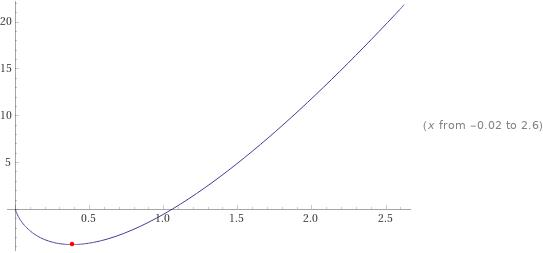
\includegraphics[width=0.5\textwidth]{images/graphic.jpeg}
\caption{График функции на исследуемом промежутке}
\end{figure}

\newpage
\section{Метод дихотомии}

В данном методе за одну итерацию рассматриваются две точки внутри исследуемого промежутка: $x_1 = x - \frac{\epsilon}{2}$ и $x_2 = x + \frac{\epsilon}{2}$, где $x$ -- середина исследуемого интервала, а сам интервал неопределенности уменьшается примерно в 2 раза. 

На каждом этапе функция вычисляется два раза -- в каждой из рассматриваемых точек, значения функций сравнивается, и исходя из этого смещаются границы интервала неопределенности.

Исследование проводится при $\epsilon = 0.0001$.

\begin{table}[h]
\begin{tabular}{|c|c|c|c|c|c|}
\hline
\rowcolor[HTML]{FFF0DB} 
\textbf{\begin{tabular}[c]{@{}c@{}}Левая \\ граница\end{tabular}} &
  \textbf{\begin{tabular}[c]{@{}c@{}}Правая \\ граница\end{tabular}} &
  \textbf{Отношение} &
  \textbf{Точка} &
  \textbf{\begin{tabular}[c]{@{}c@{}}Значение с\\ левой стороны\end{tabular}} &
  \textbf{\begin{tabular}[c]{@{}c@{}}Значение с \\ правой стороны\end{tabular}} \\ \hline
0.1     & 2.5     & --       & 1.3     & 2.56517  & 2.5663   \\ \hline
0.1     & 1.3     & 2        & 0.7     & -2.74201 & -2.74144 \\ \hline
0.1     & 0.7     & 2        & 0.4     & -3.74518 & -3.74514 \\ \hline
0.1     & 0.4     & 2        & 0.25    & -3.49678 & -3.49719 \\ \hline
0.25    & 0.4     & 2        & 0.325   & -3.70551 & -3.70566 \\ \hline
0.325   & 0.4     & 2        & 0.3625  & -3.74408 & -3.74413 \\ \hline
0.3625  & 0.4     & 2        & 0.38125 & -3.74907 & -3.74907 \\ \hline
0.38125 & 0.4     & 2        & 0.39062 & -3.74821 & -3.74819 \\ \hline
0.38125 & 0.39062 & 2.001067 & 0.38594 & -3.74891 & -3.7489  \\ \hline
0.38125 & 0.38594 & 1.997868 & 0.38359 & -3.74906 & -3.74906 \\ \hline
0.38125 & 0.38359 & 2.004274 & 0.38242 & -3.74908 & -3.74908 \\ \hline
0.38125 & 0.38242 & 2        & 0.38184 & -3.74908 & -3.74908 \\ \hline
0.38184 & 0.38242 & 2.017241 & 0.38213 & -3.74908 & -3.74908 \\ \hline
0.38213 & 0.38242 & 2        & 0.38228 & -3.74908 & -3.74908 \\ \hline
0.38213 & 0.38228 & 1.933333 & 0.3822  & -3.74908 & -3.74908 \\ \hline
\end{tabular}
\end{table}

Метод дихотомии показал, что функция на данном промежутке достигает минимума при значении $x_{min} = 0.3822021484375$, $f_{min} = -3.7490810073197856$. Выполнено 15 итераций.

\newpage
\section{Метод золотого сечения}

В данном методе отрезок, на котором рассматривается функция, делится в пропорции золотого сечения: длина всего отрезка относится к длине большей его части также, как длина большей части к меньшей.

За каждую итерацию интервал неопределенности уменьшается в $\frac{\sqrt{5}+1}{2}$ раз, эта величина постоянна. Однако со второй итерации достаточно пересчитывать значение функции только один раз по свойству золотого сечения.

Исследование проводится при $\epsilon = 0.0001$.

\begin{table}[h]
\begin{tabular}{|c|c|c|c|c|c|c|}
\hline
\rowcolor[HTML]{FFF0DB} 
\textbf{\begin{tabular}[c]{@{}c@{}}Левая\\ граница\end{tabular}} &
  \textbf{\begin{tabular}[c]{@{}c@{}}Правая\\ граница\end{tabular}} &
  \textbf{Отношение} &
  \textbf{\begin{tabular}[c]{@{}c@{}}Левая\\ точка\end{tabular}} &
  \textbf{\begin{tabular}[c]{@{}c@{}}Значение в\\ левой точке\end{tabular}} &
  \textbf{\begin{tabular}[c]{@{}c@{}}Правая\\ точка\end{tabular}} &
  \textbf{\begin{tabular}[c]{@{}c@{}}Значение в\\ правой точке\end{tabular}} \\ \hline
0.1     & 2.5     & --       & 1.01672 & -0.34828 & 1.58328 & 6.02178  \\ \hline
0.1     & 1.58328 & 1.618036 & 0.66656 & -2.92587 & --      & --       \\ \hline
0.1     & 1.01672 & 1.618029 & 0.45016 & -3.69429 & --      & --       \\ \hline
0.1     & 0.66656 & 1.618046 & 0.31641 & -3.69104 & --      & --       \\ \hline
0.31641 & 0.66656 & 1.618049 & --      & --       & 0.53282 & -3.49645 \\ \hline
0.31641 & 0.53282 & 1.617994 & 0.39907 & -3.74556 & --      & --       \\ \hline
0.31641 & 0.45016 & 1.618019 & 0.36749 & -3.74632 & --      & --       \\ \hline
0.31641 & 0.39907 & 1.618074 & 0.34798 & -3.73386 & --      & --       \\ \hline
0.34798 & 0.39907 & 1.617929 & --      & --       & 0.37955 & -3.74899 \\ \hline
0.36749 & 0.39907 & 1.617796 & --      & --       & 0.38701 & -3.74879 \\ \hline
0.36749 & 0.38701 & 1.617828 & 0.37495 & -3.74841 & --      & --       \\ \hline
0.37495 & 0.38701 & 1.618574 & --      & --       & 0.3824  & -3.74908 \\ \hline
0.37955 & 0.38701 & 1.616622 & --      & --       & 0.38416 & -3.74903 \\ \hline
0.37955 & 0.38416 & 1.618221 & 0.38131 & -3.74907 & --      & --       \\ \hline
0.38131 & 0.38416 & 1.617544 & --      & --       & 0.38307 & -3.74907 \\ \hline
0.38131 & 0.38307 & 1.619318 & 0.38199 & -3.74908 & --      & --       \\ \hline
0.38199 & 0.38307 & 1.62963  & --      & --       & 0.38266 & -3.74908 \\ \hline
0.38199 & 0.38266 & 1.61194  & 0.38224 & -3.74908 & --      & --       \\ \hline
0.38199 & 0.3824  & 1.634146 & 0.38215 & -3.74908 & --      & --       \\ \hline
0.38215 & 0.3824  & 1.64     & --      & --       & 0.3823  & -3.74908 \\ \hline
0.38215 & 0.3823  & 1.666667 & 0.38221 & -3.74908 & --      & --       \\ \hline
\end{tabular}
\end{table}

Метод золотого сечения показал, что функция на данном промежутке достигает минимума при значении $x_{min} = 0.382224424485476$, $f_{min} = -3.7490810068327103$. Выполнена 21 итерация.

\newpage
\section{Метод Фибоначчи}

Этот метод является улучшением предыдущего, в нем интервал сокращается в непостоянное количество раз.

\begin{table}[h]
\begin{tabular}{|c|c|c|c|c|c|c|}
\hline
\rowcolor[HTML]{FFF0DB} 
\textbf{\begin{tabular}[c]{@{}c@{}}Левая \\ граница\end{tabular}} &
  \textbf{\begin{tabular}[c]{@{}c@{}}Правая \\ граница\end{tabular}} &
  \textbf{Отношение} &
  \textbf{\begin{tabular}[c]{@{}c@{}}Левая \\ точка\end{tabular}} &
  \textbf{\begin{tabular}[c]{@{}c@{}}Значение в \\ левой точке\end{tabular}} &
  \textbf{\begin{tabular}[c]{@{}c@{}}Правая \\ точка\end{tabular}} &
  \textbf{\begin{tabular}[c]{@{}c@{}}Значение в \\ правой точке\end{tabular}} \\ \hline
0.1     & 2.5     & --       & 1.01672 & -0.34828 & 1.58328 & 6.02178  \\ \hline
0.1     & 1.58328 & 1.618036 & 0.66656 & -2.92587 & --      & --       \\ \hline
0.1     & 1.01672 & 1.618029 & 0.45016 & -3.69429 & --      & --       \\ \hline
0.1     & 0.66656 & 1.618046 & 0.31641 & -3.69104 & --      & --       \\ \hline
0.31641 & 0.66656 & 1.618049 & --      & --       & 0.53282 & -3.49645 \\ \hline
0.31641 & 0.53282 & 1.617994 & 0.39907 & -3.74556 & --      & --       \\ \hline
0.31641 & 0.45016 & 1.618019 & 0.36749 & -3.74632 & --      & --       \\ \hline
0.31641 & 0.39907 & 1.618074 & 0.34798 & -3.73386 & --      & --       \\ \hline
0.34798 & 0.39907 & 1.617929 & --      & --       & 0.37955 & -3.74899 \\ \hline
0.36749 & 0.39907 & 1.617796 & --      & --       & 0.38701 & -3.74879 \\ \hline
0.36749 & 0.38701 & 1.617828 & 0.37495 & -3.74841 & --      & --       \\ \hline
0.37495 & 0.38701 & 1.618574 & --      & --       & 0.3824  & -3.74908 \\ \hline
0.37955 & 0.38701 & 1.616622 & --      & --       & 0.38416 & -3.74903 \\ \hline
0.37955 & 0.38416 & 1.618221 & 0.38131 & -3.74907 & --      & --       \\ \hline
0.38131 & 0.38416 & 1.617544 & --      & --       & 0.38307 & -3.74907 \\ \hline
0.38131 & 0.38307 & 1.619318 & 0.38199 & -3.74908 & --      & --       \\ \hline
0.38199 & 0.38307 & 1.62963  & --      & --       & 0.38266 & -3.74908 \\ \hline
0.38199 & 0.38266 & 1.61194  & 0.38224 & -3.74908 & --      & --       \\ \hline
0.38199 & 0.3824  & 1.634146 & 0.38215 & -3.74908 & --      & --       \\ \hline
0.38215 & 0.3824  & 1.64     & --      & --       & 0.38231 & -3.74908 \\ \hline
0.38215 & 0.38231 & 1.5625   & 0.38221 & -3.74908 & --      & --       \\ \hline
0.38215 & 0.38224 & 1.777778 & 0.38218 & -3.74908 & --      & --       \\ \hline
0.38215 & 0.38228 & 0.692308 & --      & --       & --      & --       \\ \hline
\end{tabular}
\end{table}

Функция на данном промежутке достигает минимума при значении $x_{min} = 0.382211946017994$, $f_{min} = -3.7490810086437825$. Выполнено 22 итерации.

\newpage
\section{Метод парабол}

В данном методе функция аппроксимируется квадратичной функцией. Сравнивается минимум аппроксимирующей параболы и точка, лежащая внутри исследуемого промежутка. Исходя из значения в этих точках, можно сдвигать границы отрезка. Значение функции со второй итерации высчитывается один раз, так как второе значение сохраняется со второй итерации.

В отличие от предыдущих методов, у метода парабол суперлинейная скорость сходимости, что влияет на количество итераций. Однако эта скорость гарантируется только в малой окрестности точки минимума.

Изначально за третью точку параболы берется середина исходного промежутка, $\epsilon = 0.0001$.

\begin{table}[h]
\begin{tabular}{|c|c|c|c|c|}
\hline
\rowcolor[HTML]{FFF0DB} 
\textbf{\begin{tabular}[c]{@{}c@{}}Левая\\ граница\end{tabular}} &
  \textbf{\begin{tabular}[c]{@{}c@{}}Правая\\ граница\end{tabular}} &
  \textbf{Отношение} &
  \textbf{\begin{tabular}[c]{@{}c@{}}Минимум\\ параболы\end{tabular}} &
  \textbf{\begin{tabular}[c]{@{}c@{}}Значение \\ минимума\end{tabular}} \\ \hline
0.1       & 2.5       & --        & 0.2262186 & -3.3877692 \\ \hline
0.1       & 1.3       & 2.0000000 & 0.5272175 & -3.5139203 \\ \hline
0.2262186 & 1.3       & 1.1175459 & 0.403873  & -3.7432907 \\ \hline
0.2262186 & 0.5272175 & 3.5673931 & 0.3930555 & -3.7476161 \\ \hline
0.2262186 & 0.403873  & 1.6942947 & 0.3845723 & -3.7490111 \\ \hline
0.2262186 & 0.3930555 & 1.0648388 & 0.383205  & -3.7490686 \\ \hline
0.2262186 & 0.3845723 & 1.0535712 & 0.382467  & -3.7490802 \\ \hline
0.2262186 & 0.383205  & 1.0087097 & 0.3823075 & -3.7490809 \\ \hline
0.2262186 & 0.382467  & 1.0047232 & 0.3822391 & -3.749081  \\ \hline
0.2262186 & 0.3823075 & 1.0010219 & 0.3822217 & -3.749081  \\ \hline
0.2262186 & 0.3822391 & 1.0004384 & 0.3822152 & -3.749081  \\ \hline
0.2262186 & 0.3822217 & 1.0001115 & 0.3822133 & -3.749081  \\ \hline
0.2262186 & 0.3822152 & 1.0000417 & 0.3822127 & -3.749081  \\ \hline
0.2262186 & 0.3822133 & 1.0000122 & 0.3822125 & -3.749081  \\ \hline
0.2262186 & 0.3822127 & 1.0000038 & 0.3822124 & -3.749081  \\ \hline
0.2262186 & 0.3822125 & 1.0000013 & 0.3822124 & -3.749081  \\ \hline
0.2262186 & 0.3822124 & 1.0000006 & 0.3822124 & -3.749081  \\ \hline
0.2262186 & 0.3822124 & 1.0000001 & 0.3822124 & -3.749081  \\ \hline
0.3822124 & 0.3822124 & --        & --        & --         \\ \hline
\end{tabular}
\end{table}

Функция на данном промежутке достигает минимума при значении $x_{min} = 0.3822124198393549$, $f_{min} = -3.749081008646579$. Выполнено 18 итераций.

\newpage
\section{Комбинированный метод Брента}

Этот метод является комбинацией метода парабол и метода золотого сечения. Он пытается решить их проблемы: аппроксимирующая парабола строится с помощью трех наилучших точек (текущий минимум, точка, соответствующая второму снизу значению функции, и предыдущее значение второй точки), а минимум параболы принимается только при определенных условиях, иначе используется метод золотого сечения. 

\begin{table}[h]
\begin{tabular}{|c|c|c|c|c|}
\hline
\rowcolor[HTML]{FFF0DB} 
\textbf{\begin{tabular}[c]{@{}c@{}}Левая\\ граница\end{tabular}} &
  \textbf{\begin{tabular}[c]{@{}c@{}}Правая\\ граница\end{tabular}} &
  \textbf{Отношение} &
  \textbf{\begin{tabular}[c]{@{}c@{}}Текущий \\ минимум\end{tabular}} &
  \textbf{\begin{tabular}[c]{@{}c@{}}Значение теку- \\ щего минимума\end{tabular}} \\ \hline
0.1       & 2.5       & --       & 1.5832816 & 6.0217828 \\ \hline
0.1       & 1.5832816 & 1.618034 & 0.6665631 & 0.6665631 \\ \hline
0.1       & 1.2331263 & 1.309017 & 0.6665631 & 0.6665631 \\ \hline
0.1       & 1.0167184 & 1.236068 & 0.6665631 & 0.6665631 \\ \hline
0.1       & 0.6665631 & 1.618034 & 0.3164079 & 0.3164079 \\ \hline
0.3164079 & 0.6665631 & 1.618034 & 0.3436571 & 0.3436571 \\ \hline
0.3436571 & 0.6665631 & 1.084387 & 0.3935842 & 0.3935842 \\ \hline
0.3436571 & 0.3935842 & 6.46755  & 0.3815569 & 0.3815569 \\ \hline
0.3815569 & 0.3935842 & 4.151148 & 0.3824052 & 0.3824052 \\ \hline
0.3815569 & 0.3824052 & 14.17812 & 0.3822149 & 0.3822149 \\ \hline
0.3815569 & 0.3822149 & 1.28921  & 0.3822125 & 0.3822125 \\ \hline
0.3815569 & 0.3822125 & 1.003661 & 0.3822124 & 0.3822124 \\ \hline
0.3822124 & 0.3822125 & 655.6    & 0.3822124 & 0.3822124 \\ \hline
\end{tabular}
\end{table}

Функция на данном промежутке достигает минимума при значении $x_{min} = 0.3822124172559498$, $f_{min} = -3.7490810086465793$. Выполнено 12 итераций.

\newpage
\section{Сравнение методов}

\begin{table}[h]
\begin{tabular}{|c|c|c|c|c|c|c|}
\hline
\rowcolor[HTML]{FFF0DB} 
\textbf{$\epsilon$} &
  \textbf{$-log \epsilon$} &
  \textbf{\begin{tabular}[c]{@{}c@{}}Метод\\ дихотомии\end{tabular}} &
  \textbf{\begin{tabular}[c]{@{}c@{}}Метод золотого\\ сечения\end{tabular}} &
  \textbf{\begin{tabular}[c]{@{}c@{}}Метод\\ Фиббоначи\end{tabular}} &
  \textbf{\begin{tabular}[c]{@{}c@{}}Метод\\ парабол\end{tabular}} &
  \textbf{\begin{tabular}[c]{@{}c@{}}Метод\\ Брента\end{tabular}} \\ \hline
0.001             & 3  & 24  & 18 & 18 & 19 & 9  \\ \hline
0.0001            & 4  & 30  & 22 & 23 & 19 & 12 \\ \hline
0.00001           & 5  & 36  & 27 & 28 & 19 & 12 \\ \hline
0.000001          & 6  & 44  & 32 & 34 & 19 & 12 \\ \hline
0.0000001         & 7  & 50  & 37 & 37 & 19 & 12 \\ \hline
0.00000001        & 8  & 56  & 42 & 42 & 19 & 15 \\ \hline
0.000000001       & 9  & 64  & 46 & 47 & 23 & 21 \\ \hline
0.0000000001      & 10 & 70  & 51 & 52 & 24 & 31 \\ \hline
0.00000000001     & 11 & 76  & 56 & 57 & 26 & 38 \\ \hline
0.000000000001    & 12 & 84  & 61 & 61 & 26 & 46 \\ \hline
0.0000000000001   & 13 & 90  & 66 & 66 & 26 & 53 \\ \hline
0.00000000000001  & 14 & 96  & 70 & 71 & 26 & 62 \\ \hline
0.000000000000001 & 15 & 104 & 75 & 76 & 26 & 71 \\ \hline
\end{tabular}
\end{table}

\begin{figure}[h]
\centering
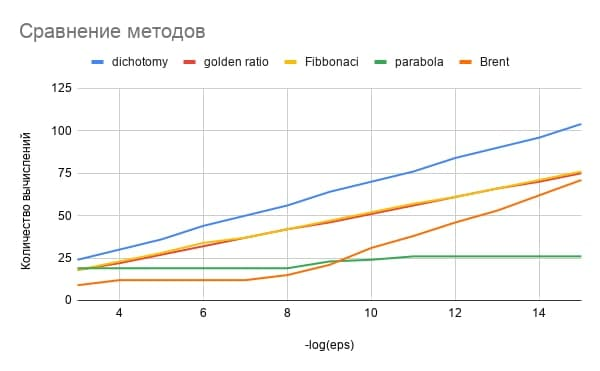
\includegraphics[width=1\textwidth]{images/new_methods.jpg}
\end{figure}

\begin{itemize}
\item Как видно из графика, для метода дихотомии требуется наибольшее количество вычислений для каждого $\epsilon$. На каждой итерации производится два вычисления функции, а длина интервала неопределенности уменьшается примерно в 2 раза. Так, например, в методах золотого сечения и Фибоначчи, интервал сокращается в меньшее количество раз, но в них не требуется дважды высчитывать функцию, что является дорогостоящей операцией.

\item Метод золотого сечения и метод Фибоначчи почти одинаковы, для них на первой итерации производится два вычисления, а далее одно. При этом для них почти не различается количество итераций относительного одинакового $\epsilon$. В сравнении с методом дихотомии, им требуется в 1,3 -- 1,4 раза меньше вычислений функций. В этих методах не требуется вычислять значение функции на границах промежутка, а значит, ими удобно исследовать функции с ассимптотами. Они имеют линейную скорость сходимости, поэтому требуется большее количество итераций, чем для методов параболы и Брента.

\item Метод парабол имеет суперлинейную скорость сходимости, поэтому ему требуется меньшее количество итераций. При этом на каждой итерации, кроме первой, высчитывается одно значение -- значение в минимуме аппроксимирующей параболы. Однако, на первых шагах этот метод нестабилен, интервал неопределенности либо слишком сильно, либо слабо сокращается. Зато достигнув малой окрестности $x_{min}$, достигается высокая точность, поэтому для разных $\epsilon$ требуется одинаковое количество итераций. Также, для вычисления первого минимума параболы требуется посчитать значение функции в крайних точках интервала, что невозможно сделать, если через них проходит ассимптоты функции.

\item Метод Брента является комбинацией метода золотого сечения и парабол. В нем компенсируются недостатки этих методов: большое количество итераций золотого сечения и неустойчивость парабол. Как и в предыдущих трех методах, на каждой итерации, помимо первой, высчитывается только одно значение функции. Из графика видно, что удалось по количеству итераций и запросов к функции улучшить метод золотого сечения, однако метод парабол все еще работает лучше. 
\end{itemize}

\newpage
\section{Работа алгоритмов на многомодальных функциях}

Была рассмотрена работа алгоритмов на унимодальных функциях -- функциях, непрерывных на исследуемом промежутке $[a, b]$ и на которых существует такая точка $x_0$, что $f(x_0)$ в полуинтервале $[a, x_0)$ убывает, а в $(x_0, b]$ возрастает. Но на многомодальных функциях, то есть функциях, имеющих несколько локальных минимумов на исследуемом интервале, минимизация данными алгоритмами затрудняется.

Примеры исследования многомодальных функций:

\begin{enumerate}
\item $x^4 - 8 \cdot x^3 + 22 \cdot x^2 - 24 \cdot x + 1$ на интервале $[0; 5]$ 

\begin{figure}[h]
\centering
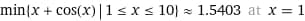
\includegraphics[width=0.4\textwidth]{images/2loc1.jpg} \\
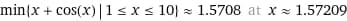
\includegraphics[width=0.4\textwidth]{images/2loc2.jpg}
\caption{Найденное решение}
\end{figure}

\begin{figure}[h]
\centering
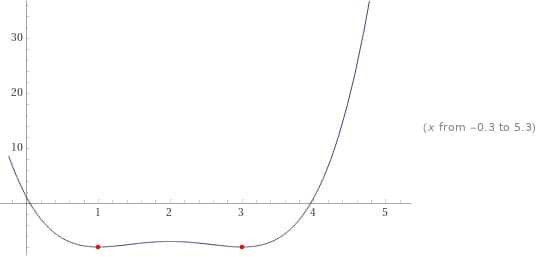
\includegraphics[width=0.4\textwidth]{images/1loc3.jpg}
\caption{График функции на исследуемом промежутке}
\end{figure}

\begin{table}[h]
\begin{tabular}{|
>{\columncolor[HTML]{FFF0DB}}c |c|c|c|}
\hline
 &
  \cellcolor[HTML]{FFF0DB}\textbf{\begin{tabular}[c]{@{}c@{}}Количество\\ вычислений\end{tabular}} &
  \cellcolor[HTML]{FFF0DB}\textbf{\begin{tabular}[c]{@{}c@{}}Точка \\ минимума\end{tabular}} &
  \cellcolor[HTML]{FFF0DB}\textbf{\begin{tabular}[c]{@{}c@{}}Значение\\ минимума\end{tabular}} \\ \hline
\textbf{\begin{tabular}[c]{@{}c@{}}Метод\\ дихотомии\end{tabular}}              & 32 & 2.9999542236328125 & -7.999999991618495 \\ \hline
\textbf{\begin{tabular}[c]{@{}c@{}}Метод\\ золотого сечения\end{tabular}}       & 23 & 2.9999910587085203 & -7.999999999680227 \\ \hline
\textbf{\begin{tabular}[c]{@{}c@{}}Метод\\ Фибоначчи\end{tabular}}              & 25 & 3.0000305470985342 & -7.999999996267363 \\ \hline
\textbf{\begin{tabular}[c]{@{}c@{}}Метод\\ парабол\end{tabular}}                & 87 & 2.999999801466867  & -7.999999999999858 \\ \hline
\textbf{\begin{tabular}[c]{@{}c@{}}Комбинированный\\ метод Брента\end{tabular}} & 17 & 3.0000000233999984 & -8.0               \\ \hline
\end{tabular}
\end{table}

В этом примере все пять методов попали в одинаковый локальный минимум. Методу Брента потребовалось меньше всего итераций и вычислений, он оказался наиболее устойчивым. Заметно, что метод парабол перестал быть оптимальным, ему потребовалось наибольшее количество итераций. Это связано со сравнением минимума промежуточной аппроксимирующей параболы и третьей точки, так как есть несколько интервалов, для которых выполняется условие унимодальности.

\newpage
\item $x+cos(x)$ на интервале $[1; 10]$

\begin{figure}[h]
\centering
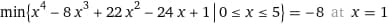
\includegraphics[width=0.4\textwidth]{images/1loc1.jpg} \\
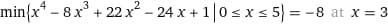
\includegraphics[width=0.4\textwidth]{images/1loc2.jpg}
\caption{Найденное решение}
\end{figure}

\begin{figure}[h]
\centering
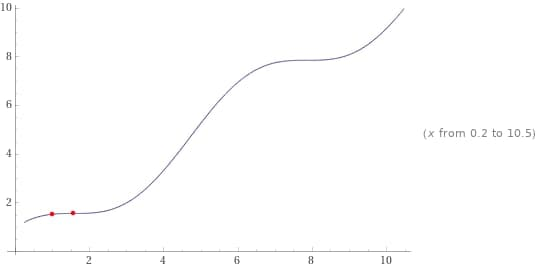
\includegraphics[width=0.4\textwidth]{images/2loc3.jpg}
\caption{График функции на исследуемом промежутке}
\end{figure}

\begin{table}[ht]
\begin{tabular}{|
>{\columncolor[HTML]{FFF0DB}}c |c|c|c|}
\hline
 &
  \cellcolor[HTML]{FFF0DB}\textbf{\begin{tabular}[c]{@{}c@{}}Количество\\ вычислений\end{tabular}} &
  \cellcolor[HTML]{FFF0DB}\textbf{\begin{tabular}[c]{@{}c@{}}Точка \\ минимума\end{tabular}} &
  \cellcolor[HTML]{FFF0DB}\textbf{\begin{tabular}[c]{@{}c@{}}Значение\\ минимума\end{tabular}} \\ \hline
\textbf{\begin{tabular}[c]{@{}c@{}}Метод\\ дихотомии\end{tabular}}              & 34  & 1.0000686645507812 & 1.5403131899180849 \\ \hline
\textbf{\begin{tabular}[c]{@{}c@{}}Метод\\ золотого сечения\end{tabular}}       & 24  & 1.000070225814992  & 1.540313437365185  \\ \hline
\textbf{\begin{tabular}[c]{@{}c@{}}Метод\\ Фибоначчи\end{tabular}}              & 26  & 1.0000566374354567 & 1.5403112836784405 \\ \hline
\textbf{\begin{tabular}[c]{@{}c@{}}Метод\\ парабол\end{tabular}}                & 139 & 5.5                & 6.20866977429126   \\ \hline
\textbf{\begin{tabular}[c]{@{}c@{}}Комбинированный\\ метод Брента\end{tabular}} & 56  & 1.000037734178906  & 1.5403082874457086 \\ \hline
\end{tabular}
\end{table}

В этом случае четыре метода попали в одинаковую точку, однако методу Брента потребовалось большее количество вычислений и итераций, чем остальным, кроме парабол. Методам золотого сечения и Фибоначчи все так же требуется примерно одинаковое количество вычислений, как было и для унимодальных функций. Количество вычислений метода парабол значительно отличается от остальных, и он не попал в минимум. Это связано с тем, что один из локальных минимумов находится на конце рассматриваемого интервала. Из-за проблем с методом парабол в этом примере так изменилась устойчивость метода Брента.

\newpage
\item $sin(x)$ на интервале $[0; 15]$

\begin{figure}[h]
\centering
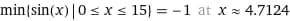
\includegraphics[width=0.4\textwidth]{images/3loc1.jpg} \\
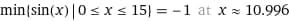
\includegraphics[width=0.4\textwidth]{images/3loc2.jpg}
\caption{Найденное решение}
\end{figure}

\begin{figure}[h]
\centering
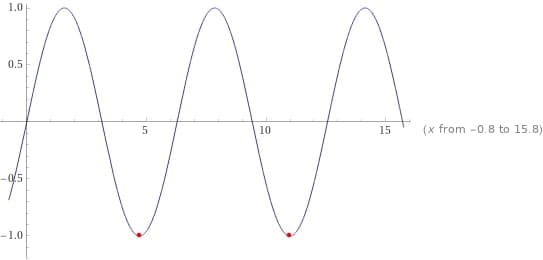
\includegraphics[width=0.4\textwidth]{images/3loc3.jpg}
\caption{График функции на исследуемом промежутке}
\end{figure}

\begin{table}[h]
\begin{tabular}{|
>{\columncolor[HTML]{FFF0DB}}c |c|c|c|}
\hline
 &
  \cellcolor[HTML]{FFF0DB}\textbf{\begin{tabular}[c]{@{}c@{}}Количество\\ вычислений\end{tabular}} &
  \cellcolor[HTML]{FFF0DB}\textbf{\begin{tabular}[c]{@{}c@{}}Точка \\ минимума\end{tabular}} &
  \cellcolor[HTML]{FFF0DB}\textbf{\begin{tabular}[c]{@{}c@{}}Значение\\ минимума\end{tabular}} \\ \hline
\textbf{\begin{tabular}[c]{@{}c@{}}Метод\\ дихотомии\end{tabular}}              & 36 & 4.712390899658203  & -0.9999999999981581 \\ \hline
\textbf{\begin{tabular}[c]{@{}c@{}}Метод\\ золотого сечения\end{tabular}}       & 25 & 4.712351389414225  & -0.9999999992934595 \\ \hline
\textbf{\begin{tabular}[c]{@{}c@{}}Метод\\ Фибоначчи\end{tabular}}              & 27 & 4.7124009175873    & -0.9999999999287515 \\ \hline
\textbf{\begin{tabular}[c]{@{}c@{}}Метод\\ парабол\end{tabular}}                & 12 & 10.995574284025212 & -1.0                \\ \hline
\textbf{\begin{tabular}[c]{@{}c@{}}Комбинированный\\ метод Брента\end{tabular}} & 11 & 4.712388980353899  & -1.0                \\ \hline
\end{tabular}
\end{table}

В этой функции методы дихотомии, золотого сечения, Фибоначчи и Брента попали в левый локальный минимум, а метод парабол в правый. Методу Брента и парабол потребовалось наименьшее количество вычислений.

\end{enumerate}

\newpage
\section{Выводы}

В ходе лабораторной работы были исследованы пять методов одномерной оптимизации на унимодальных и многомодальных функциях. 

На унимодальных функциях лучше всего показал себя метод парабол, ему требовалось наименьшее количество вычислений, что важно с точки зрения стоимости операции. Однако этот метод оказался самым нестабильным, так как он ведет себя хорошо только в окрестности минимума, а сначала делает неравномерные шаги. Разница между методом золотого сечения и методом Фибоначчи почти не заметна, делается только одно вычисление на каждой итерации. Метод дихотомии действует по такому же принципу, как и эти методы, деля отрезок, но в нем требуется два вычисления на каждом этапе, что не выгодно, но само количество итераций на нем меньше. Комбинация метода золотого сечения и парабол -- метод Брента, оказался самым устойчивым, но в нем требуется большее количество итераций, чем в методе парабол.

На многомодальных функциях хуже всего ведет себя метод парабол из-за своей неустойчивости, а лучше всего -- метод Брента. Исследование функций с несколькими локальными минимумами/максимумами на промежутке затруднительно с помощью данных методов оптимизации.

Реализация: \href{https://github.com/Mr3zee/ITMO-Optimization-Methods-LAB1-2021/}{GitHub}.

\end{document}